\documentclass[11pt,a4paper]{article}
\usepackage{fontspec}
\setmainfont{TeX Gyre Pagella}
\newfontfamily\headfont{Inter}[UprightFont=*-ExtraBold,BoldFont=*-ExtraBold,Extension=.otf,Path=/usr/share/fonts/opentype/inter/]
\usepackage[a4paper,margin=2.3cm]{geometry}
\usepackage{graphicx,booktabs,float,caption,array,xcolor,longtable}
\usepackage{xurl}
\usepackage[hidelinks]{hyperref}
\usepackage{titlesec}
\usepackage[round]{natbib}
\usepackage{setspace}
\setstretch{1.05}
\renewcommand{\topfraction}{0.9}
\renewcommand{\bottomfraction}{0.8}
\renewcommand{\textfraction}{0.1}
\renewcommand{\floatpagefraction}{0.75}
\setlength{\parindent}{0pt}
\setlength{\parskip}{0.55em}
\titleformat{\section}{\headfont\Large}{\thesection}{0.8em}{}
\titleformat{\subsection}{\headfont\large}{\thesubsection}{0.8em}{}
\captionsetup{font=small,labelfont=bf}
\urlstyle{same}
\hypersetup{pdftitle={Where the Wolves Were},pdfauthor={Tristan Hotham}}

\newcolumntype{R}[1]{>{\raggedright\arraybackslash}p{#1}}
\begin{document}
\begin{center}
{\Large\bfseries Where the Wolves Were\par}
\vspace{0.4em}
{\large Animals in the place names of Britain and Ireland, from a national gazetteer checked name by name\par}
\vspace{1.2em}
{\large Tristan Hotham\par}
\vspace{0.3em}
{\small Independent researcher\\
ORCID: 0000-0003-4931-9349\\
DOI: https://doi.org/10.5281/zenodo.24075293\par}
\vspace{0.8em}
2026
\end{center}

\begin{quote}
\small
\begin{center}\textbf{Abstract}\end{center}
Place names keep animals long after the animals have gone. I search 145,934 named points from OpenStreetMap (places in the United Kingdom and Ireland, and named hills, woods, cliffs, springs and bays in the United Kingdom) for animal elements in Old English, Old Norse, Welsh, Scottish Gaelic, Irish and later English and Scots, using a conservative, documented word list: whole settlement names whose etymology the standard dictionaries give, the ordinary Celtic-language words for each animal inside each language's area, and English and Scots animal words only beside a landscape word. Of 800 candidates, 30 were removed as known false friends and 26 more on reading every candidate by hand (7.0\% in all), leaving 662 places once repeats of a name within 3 km are merged, 189 of them with a certain reading. Wolf names (33) lie at a median 256 m above sea level against 103 m for random names of the same kinds, and most later wolf names are crags and cleughs in the northern hills; boar and deer names stand high too, otter names low. Crane names (23) are English but neither low-lying nor concentrated in the Fens. Eagle names are 68.3\% Gaelic, Welsh or Irish, and raven, boar and eagle names survive mainly in Gaelic, while fox and deer names are mainly later English. The old English names on the map were formed while wolves, beavers, cranes and boar still lived here, and have outlived them by four to eight centuries.

\textbf{Keywords:} place names; toponymy; historical ecology; extinct species; wolf; beaver; crane; OpenStreetMap; Old English; Gaelic; Welsh
\end{quote}

\section{Introduction}
Wolves were gone from England by around 1500, beavers by the sixteenth century at the latest, cranes stopped breeding around 1600 and wild boar had left the wild by the thirteenth century \citep{yalden1999,coles2006,boisseau1998,pluskowski2006}. Place names are one of the few records that place these animals in the landscape of the early medieval centuries. Aybes and Yalden used the English Place-Name Society's county surveys to map the place names of wolves and beavers \citep{aybes1995}, and Boisseau and Yalden did the same for the crane \citep{boisseau1998}. Those studies read the scholarly surveys county by county. This paper asks a simpler and more open question of a modern open gazetteer: across Britain and Ireland, which named places and hills keep an animal in their name, in which languages, and where?

The answer depends on care with false friends. Wolverhampton is named after a woman, Wulfrun; Eagle in Lincolnshire is an oak wood; Swanage is the farm of herdsmen; many \textit{Brock-} names are brooks, and many Irish \textit{Cran-} names are trees. So the method is conservative, every rule is written down, and every candidate was read by eye.

\section{Data}
\textbf{Names.} Three OpenStreetMap extracts, queried with QLever \citep{bast2017}: 106,905 place nodes in the United Kingdom (city, town, village, hamlet, suburb, neighbourhood, quarter, locality, farm and isolated dwelling) with \texttt{name}, \texttt{name:cy} and \texttt{name:gd}; 24,964 named natural features in the United Kingdom (peaks, hills, ridges, valleys, woods, cliffs, springs, bays and an island); and 14,065 place nodes in Ireland with \texttt{name:ga}. Each point is assigned a county and nation from the ONS boundaries and a ground height from the AWS Terrain Tiles at zoom 10 (about 90 m).

\textbf{Etymologies.} English and Norse settlement names follow the standard dictionaries \citep{mills2011,watts2004,ekwall1960} with \citet{gelling2000} on the landscape words; Welsh, Gaelic and Irish words are read in their ordinary dictionary sense, with \citet{owen2007} and \citet{watson1926} for the place-name patterns.

\section{Method}
\textbf{Three kinds of rule} (\texttt{code/elements.py}, \texttt{data/elements.csv}). (1) \textit{Named}: 69 English or Norse settlement names that the dictionaries explain with an animal (Table~\ref{tab:named}), matched as whole names with optional prefixes such as Great or Upper and a short list of suffixes (Abbey, Common, Green, Heath, a saint's name), only on settlements, and only in the county of the dictionary's place where that is known. Names that recur (Hartley, Woolley, Foxley) are marked probable outside the county I am sure of. (2) \textit{Word}: 37 rules for the Welsh, Scottish Gaelic and Irish words for each animal, with their mutated and genitive forms (Welsh \textit{blaidd}, \textit{bleiddiaid}; Gaelic \textit{iolair}, \textit{na h-iolaire}; \textit{fitheach}, \textit{an fhithich}; Irish \textit{broc}, \textit{na mbroc}), applied to \texttt{name} and the language tag, inside Wales, Scotland or Ireland respectively. (3) \textit{Modern}: 22 rules for English and Scots animal words (wolf, eagle, raven, crane, hart, hind, deer, stag, brock, badger, fox, tod, cat, otter, swan, kite, glede, boar), only followed by a landscape word (crag, hill, knowe, cleugh, hole, scar, nest, tor, law and others), and never on farms, single houses or modern suburbs. Gaelic \textit{madadh} alone can be a dog, a fox or a wolf; its 23 names are kept apart and not counted.

\textbf{False friends and review.} 23 exclusion patterns remove known false friends (Table~\ref{tab:ff}). I then read all 800 candidates and dropped or corrected 26 more in a documented overrides file, for example Donnybrook (Domhnach Broc, St Broc's church), Brackagh (usually Irish \textit{breacach}, speckled), Colmonell (St Colm\'an Ela), Arbirlot (the Elliot Water), and inn signs such as Stags Head. Rules changed in review too: \textit{buck} was removed because Old English \textit{bucc} can be a he-goat, and \textit{roe} because Roedean is a rough valley. In all 7.0\% of candidates were removed. Every candidate, with the reason it was kept or dropped, is in \texttt{data/candidates\_review.csv}.

\textbf{Places.} Repeats of one name for one animal within 3 km (Woolpit, Woolpit Green, Woolpit Heath) are counted as one place (82 names merged), leaving 662 places.

\textbf{Height test.} For each animal, the median ground height of its UK places is compared with the median of random UK names of the same kinds (the same numbers of peaks, villages, localities and so on), drawn 20,000 times; the one-sided p-value is the share of draws at least as high (or as low).

\section{Results}
\subsection{The animals}
Table~\ref{tab:animals} gives the places for each animal. Deer (150), fox (147) and raven (93) lead; wolf has 33, eagle 41, crane 23, wild boar 22 and beaver only 3. By language, 95 places are Old English, 3 Old Norse, 23 Welsh, 128 Scottish Gaelic, 23 Irish and 390 later English or Scots. 189 (28.5\%) have a certain reading.

\begin{table}[tbp]\centering\footnotesize\setlength{\tabcolsep}{4pt}\caption{Places by animal: total, with a certain reading, by language (Old English, Old Norse, Welsh, Scottish Gaelic, Irish, later English or Scots), and the median ground height (m) of UK places against that expected for random names of the same kinds, with the one-sided p-value (+ higher, $-$ lower than expected; 20,000 draws).}\label{tab:animals}\begin{tabular}{lrrrrrrrrrrr}\toprule Animal & Places & Certain & OE & ON & Wel & Gae & Ir & Later & Height & Expected & p\\\midrule
Deer & 150 & 47 & 33 & 0 & 7 & 28 & 2 & 80 & 252 & 136 & 0.000+\\
Fox & 147 & 22 & 14 & 0 & 5 & 9 & 2 & 117 & 144 & 123 & 0.104+\\
Raven & 93 & 38 & 0 & 0 & 2 & 36 & 0 & 55 & 224 & 169 & 0.025+\\
Badger & 59 & 6 & 3 & 0 & 0 & 3 & 17 & 36 & 141 & 129 & 0.342+\\
Wildcat & 55 & 1 & 4 & 0 & 1 & 9 & 1 & 40 & 202 & 135 & 0.015+\\
Eagle & 41 & 31 & 6 & 0 & 4 & 23 & 1 & 7 & 230 & 216 & 0.378+\\
Wolf & 33 & 4 & 8 & 1 & 3 & 0 & 0 & 21 & 256 & 103 & 0.000+\\
Crane & 23 & 9 & 11 & 1 & 0 & 0 & 0 & 11 & 103 & 86 & 0.240+\\
Wild boar & 22 & 17 & 5 & 0 & 0 & 15 & 0 & 2 & 334 & 129 & 0.000+\\
Otter & 15 & 9 & 5 & 0 & 1 & 3 & 0 & 6 & 36 & 73 & 0.052$-$\\
Swan & 9 & 1 & 2 & 0 & 0 & 1 & 0 & 6 & & &\\
Kite & 9 & 0 & 1 & 0 & 0 & 0 & 0 & 8 & & &\\
Beaver & 3 & 2 & 3 & 0 & 0 & 0 & 0 & 0 & & &\\
Salmon & 3 & 2 & 0 & 1 & 0 & 1 & 0 & 1 & & &\\
\bottomrule\end{tabular}\end{table}

\begin{figure}[tbp]\centering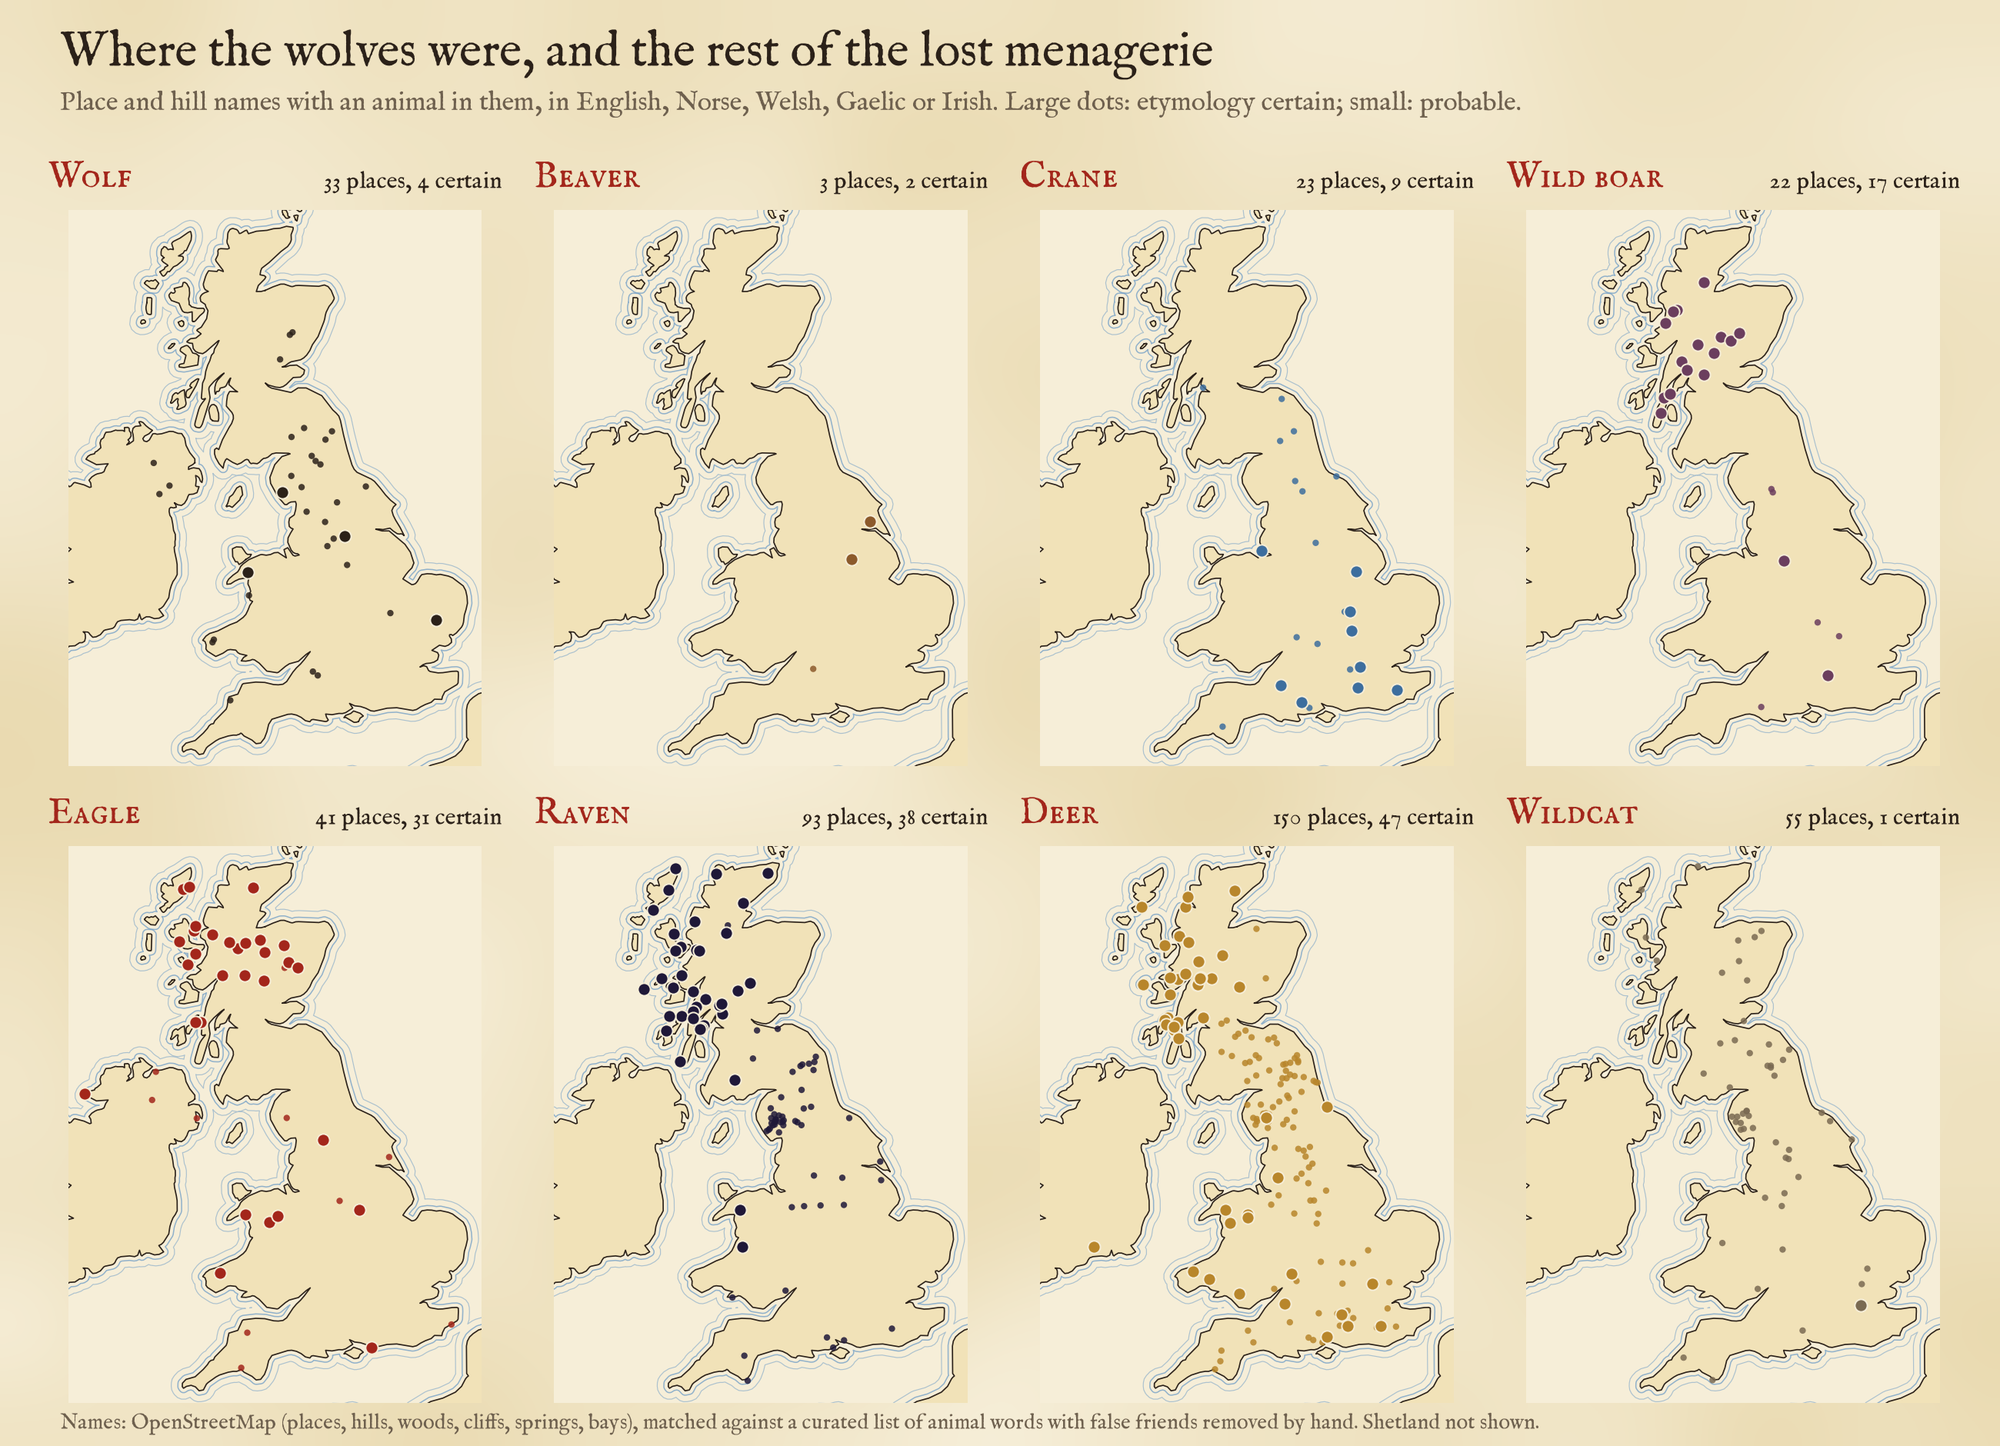
\includegraphics[width=\textwidth]{f_animals.png}
\caption{Places named for eight animals. Large dots: certain reading; small: probable.}\label{fig:animals}\end{figure}

\subsection{Wolves in the uplands}
The certain wolf names are few: Woolpit in Suffolk (Old English \textit{wulf-pytt}, a pit for trapping wolves), Woolley in West Yorkshire, Ulpha in Cumbria (Old Norse \textit{ulfr} and \textit{haugr}) and Welsh Cwm Bleiddiaid. A farm called simply Blaidd is kept as probable, since a one-word house name may be modern. Most wolf names are later English and Scots names of crags, cleughs and holes: 73.3\% of the 30 English-language wolf names lie north of 53.5\textdegree{}N. The median wolf place stands at 256 m, against 103 m expected for names of the same kinds; no random draw was as high (p $<$ 0.0001). Because the descriptive rules accept only names with a landscape word, the draw from all names of a kind flatters every animal named in that way; among the descriptive English and Scots names alone, wolf names stand at a median 289 m against 224 m for all such names, and against the other animals' kept names of the same kind and rule family (old or descriptive) the wolf names are still higher (148 m expected, p = 0.003). Wild boar (334 m against 129 m) and deer (252 m against 136 m) are also high; ravens (p = 0.02) and wildcats (p = 0.01) somewhat high; fox (p = 0.10), badger, eagle and crane names lie about where expected, and otter names low (36 m against 73 m, p = 0.05; 0.02 against other animals' names), as expected for a river animal, though with only 15 places the result is weak.

\begin{figure}[tbp]\centering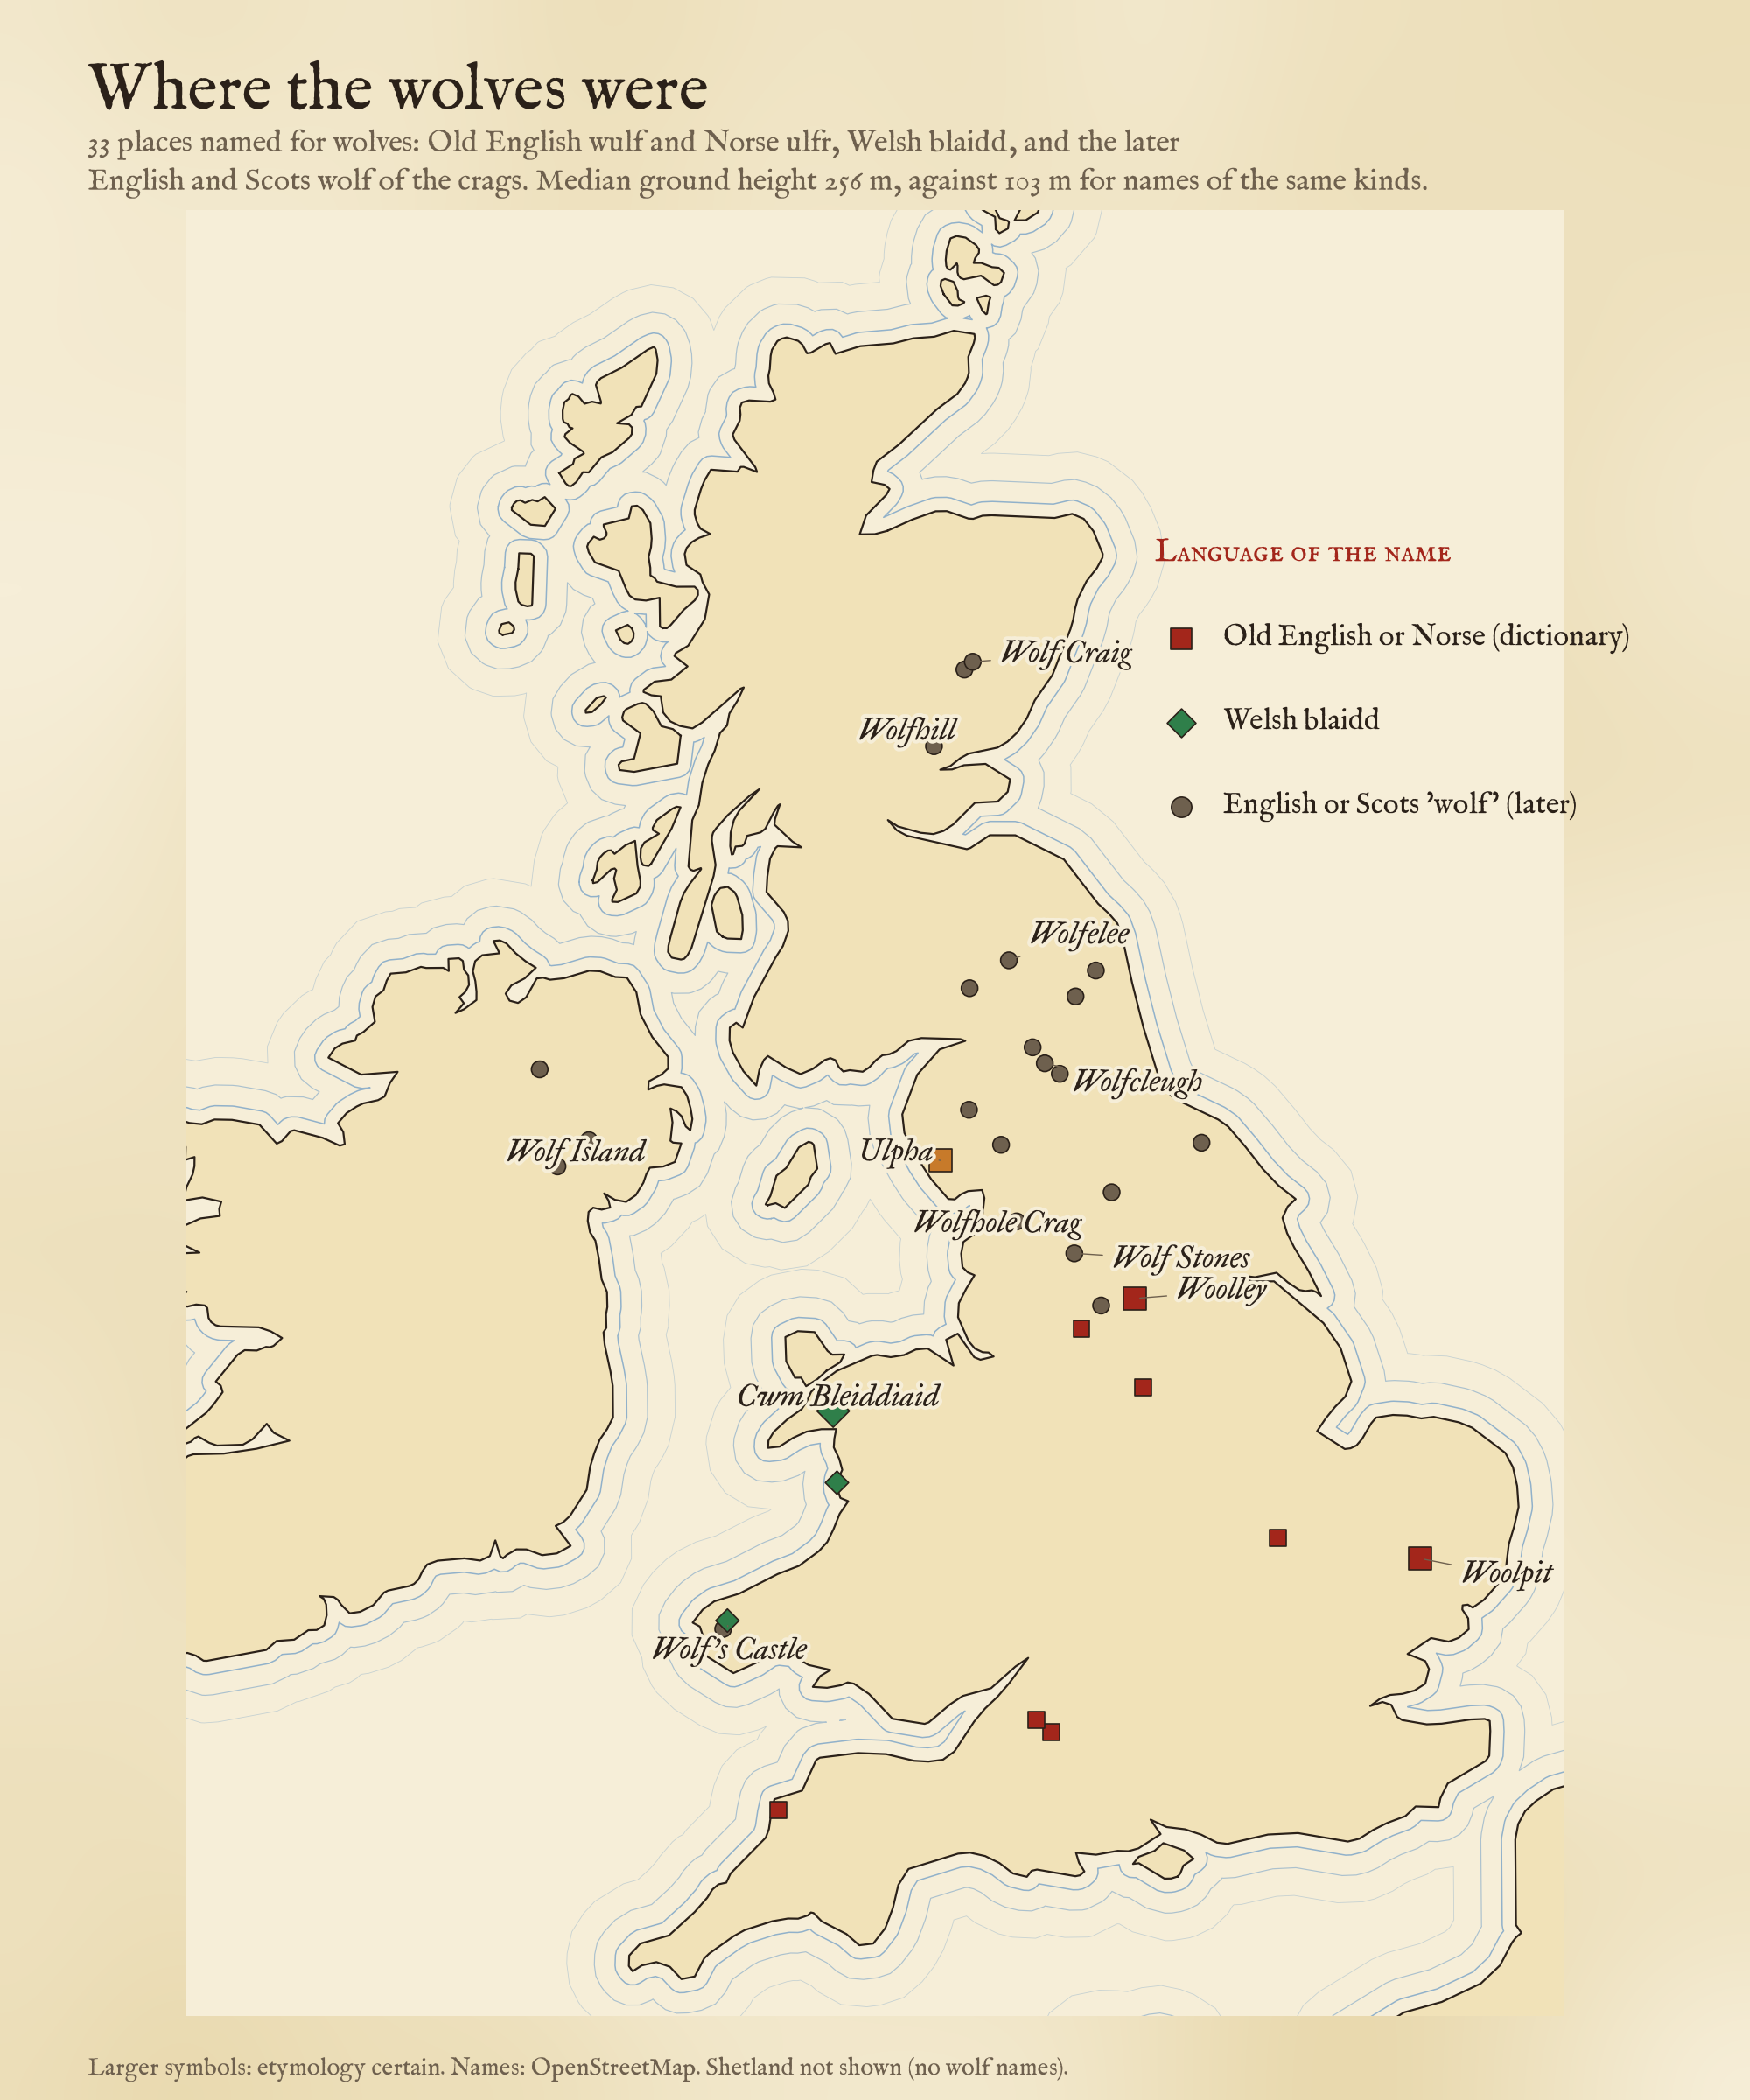
\includegraphics[width=0.8\textwidth]{f_wolves.png}
\caption{Wolf names by language.}\label{fig:wolves}\end{figure}

\begin{figure}[tbp]\centering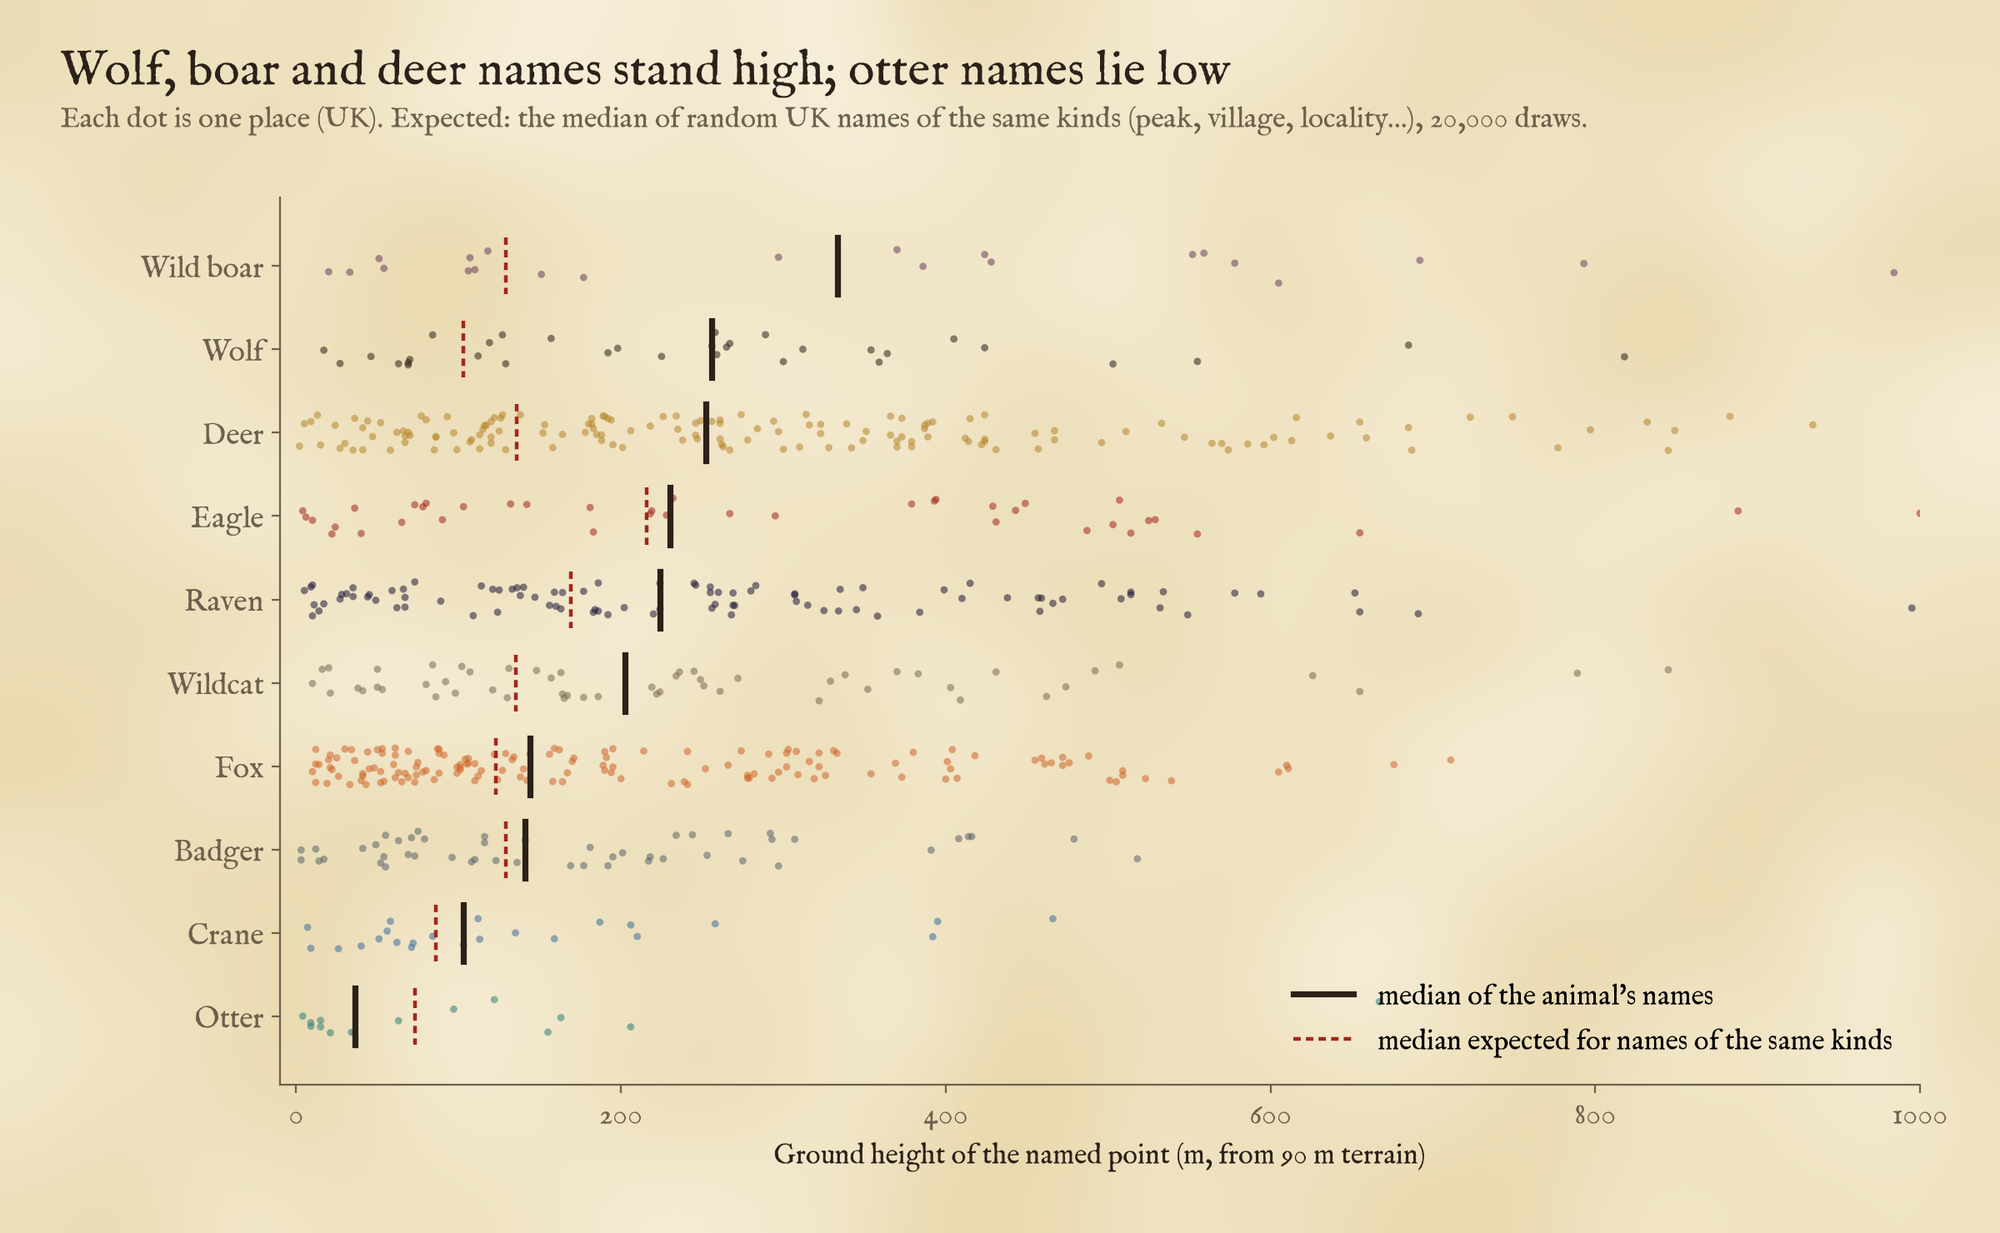
\includegraphics[width=\textwidth]{f_height.png}
\caption{Ground height of each UK place by animal: median (black) and the median expected for random names of the same kinds (red, dashed).}\label{fig:height}\end{figure}

\subsection{Cranes and beavers}
The crane names are 91.3\% English: Cranfield, Cranbrook, Cranborne, Cranford, Cranmore, Cranwell, Cranleigh and Norse Tranmere. Old English \textit{cran} may also have meant the heron, and the dictionaries often gloss it so. They are not concentrated in the Fens: only 1 lies in Cambridgeshire, Lincolnshire, Norfolk or Suffolk, and their median height (103 m) is close to that expected (86 m, p = 0.77 for lower). The beaver leaves only Beverley, Bevercotes and Beversbrook in this gazetteer, far fewer than the field and minor names found in the county surveys \citep{aybes1995}.

\subsection{Languages}
Animals differ in the language that keeps them (Figure~\ref{fig:layers}). Eagle names are 68.3\% Gaelic, Welsh or Irish (23 Gaelic \textit{iolair}, 4 Welsh \textit{eryr}, 1 Irish \textit{iolar}) and only 6 Old English \textit{earn}: Arncliffe, Earnley, Arnold, Yarnscombe and Ernesettle. Raven names are Gaelic \textit{fitheach} in the west Highlands and English crag names in the north of England (58.2\% of the English ones in Cumbria and Northumberland). Boar names are mostly Gaelic \textit{tuirc} hills. Fox and deer, animals that never left, are named mostly in later English and Scots.

\begin{figure}[tbp]\centering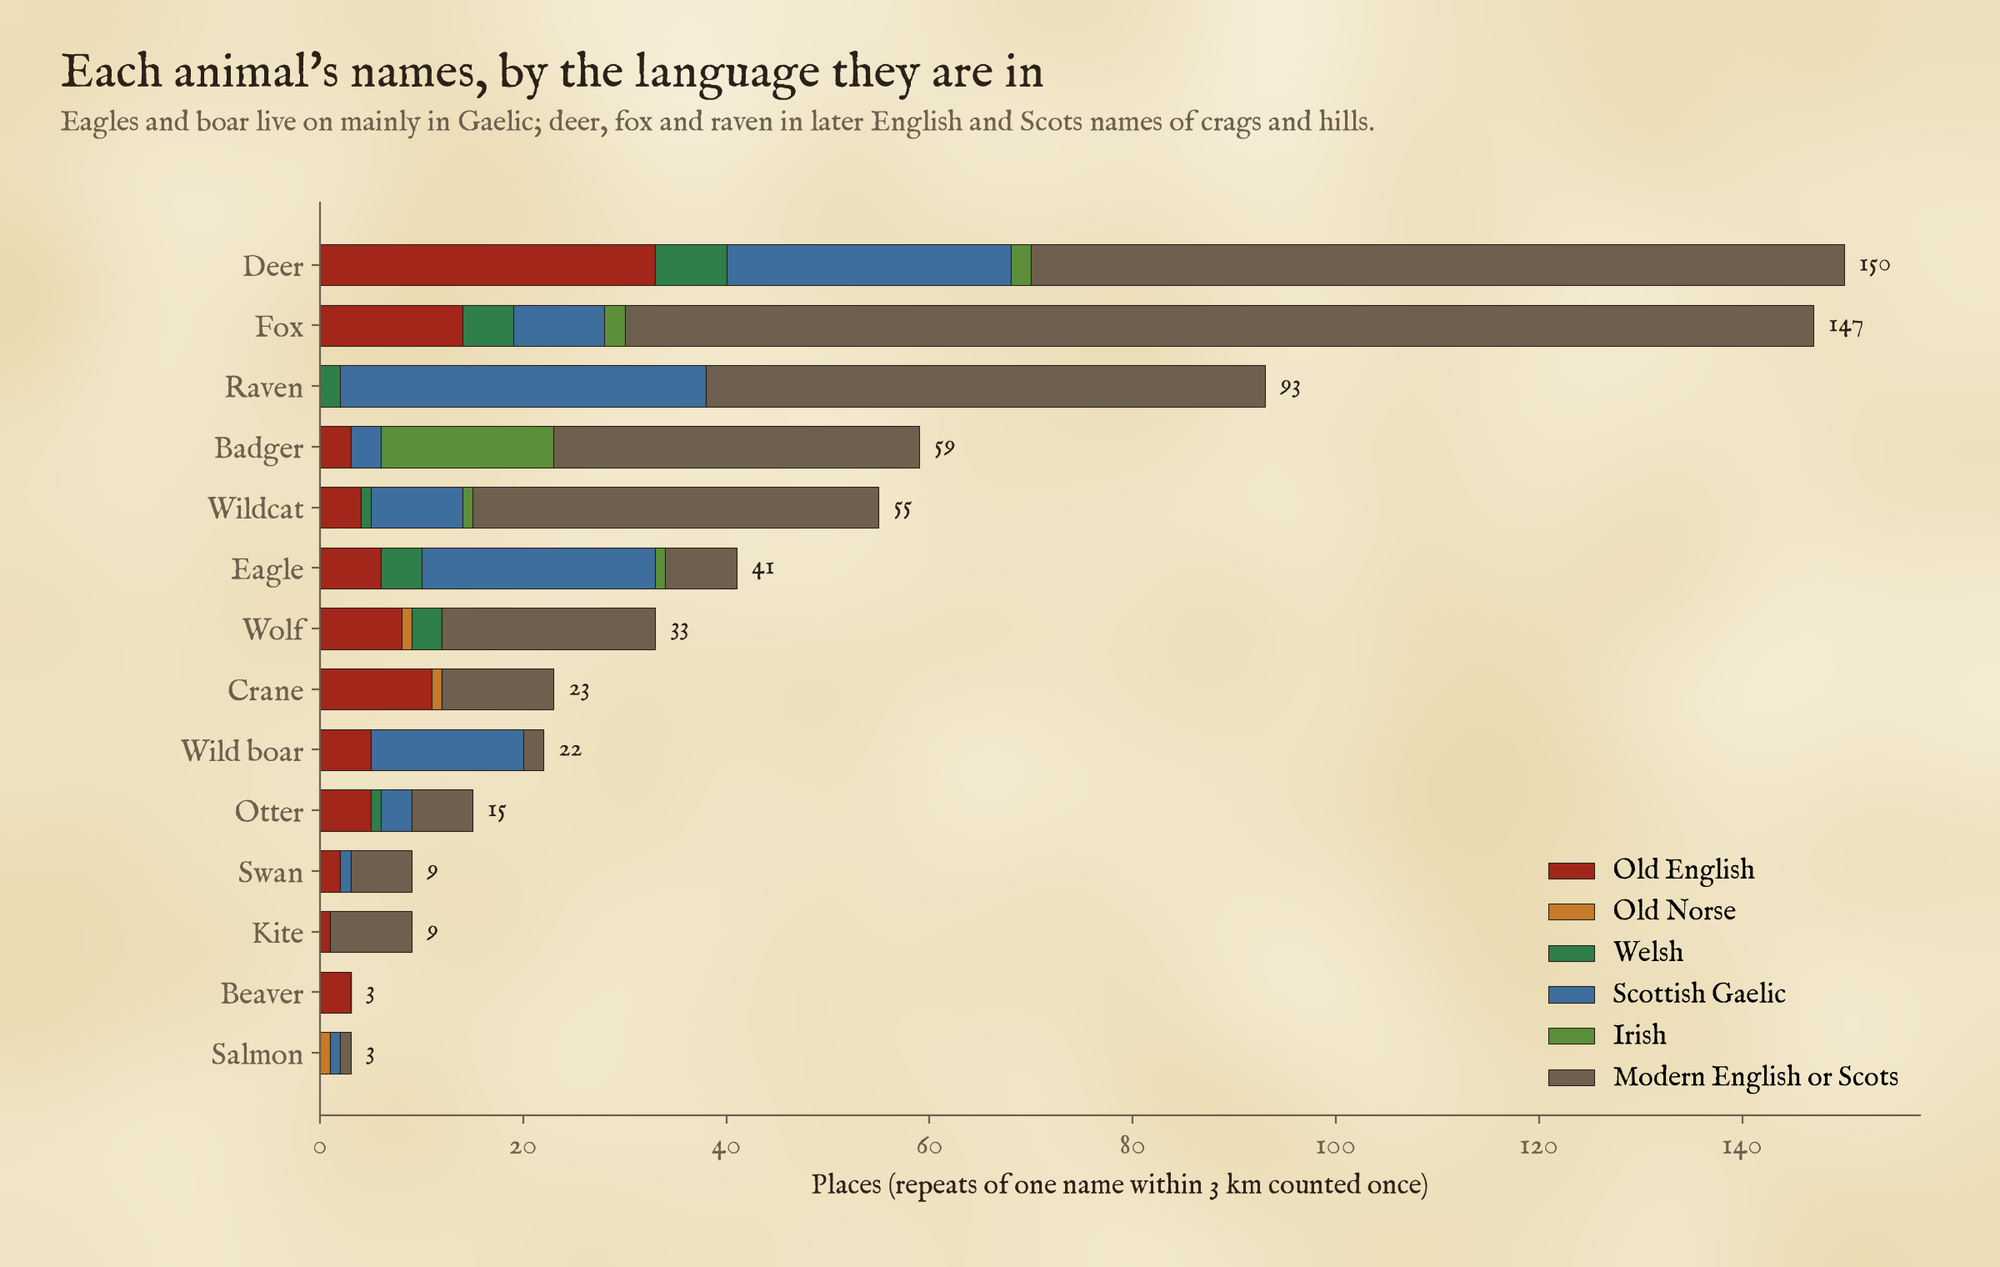
\includegraphics[width=\textwidth]{f_layers.png}
\caption{Places by animal and language.}\label{fig:layers}\end{figure}

\begin{figure}[tbp]\centering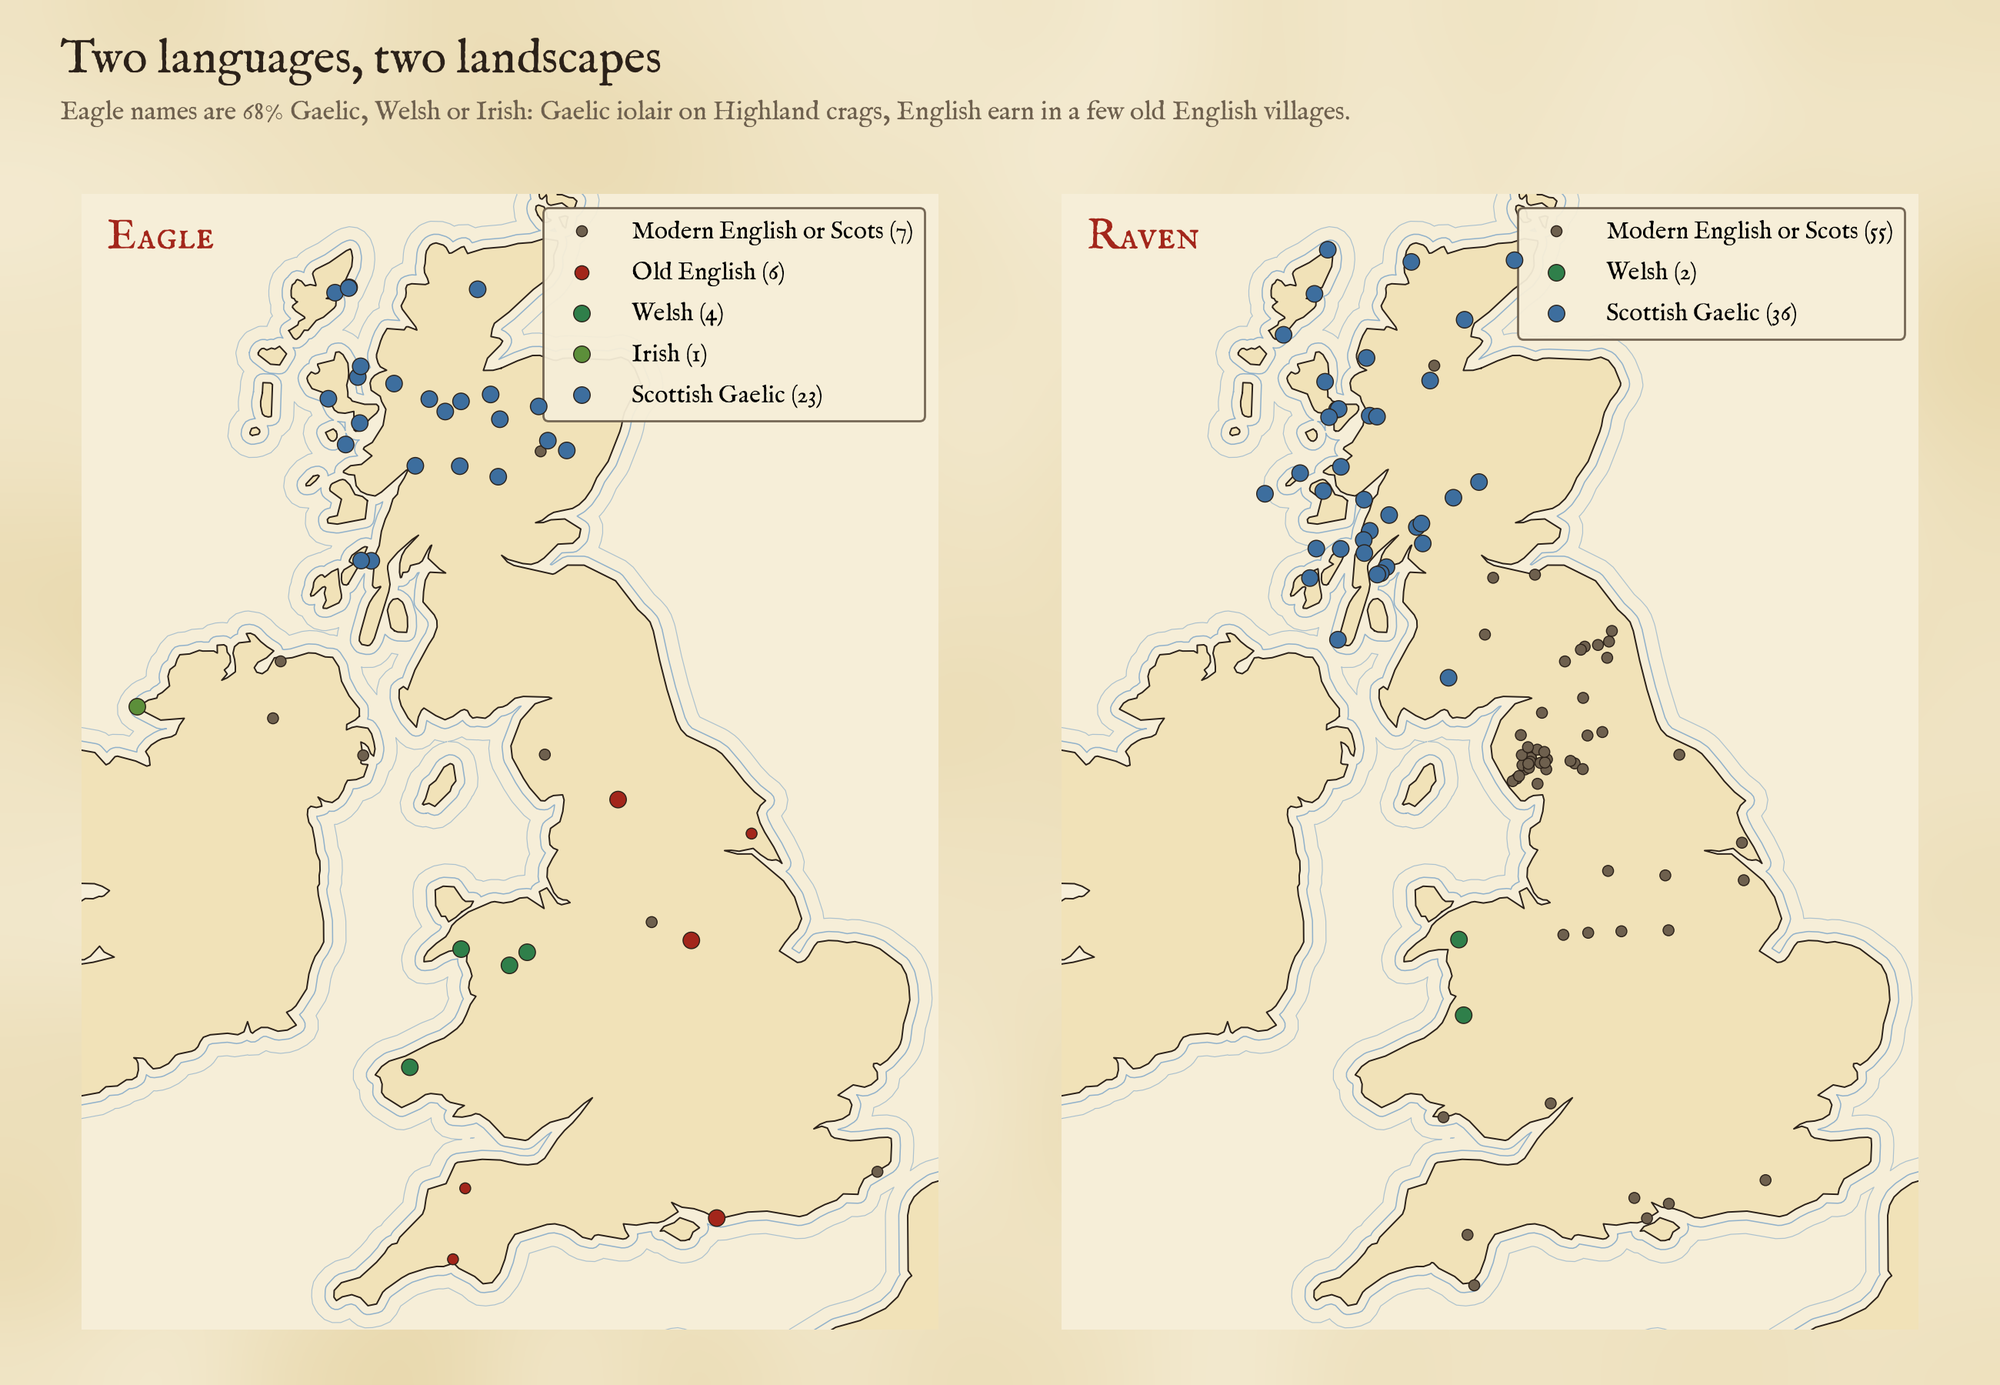
\includegraphics[width=\textwidth]{f_eagles.png}
\caption{Eagle and raven names by language.}\label{fig:eagles}\end{figure}

\subsection{Where names are densest}
One 10 km square of the British National Grid in Cumbria, in the fells around Dunnerdale, holds names for 4 animals. By county, Northumberland has 16.0 animal places per 1,000 named points, Argyll and Bute 13.2 and Cumbria 11.2 (counties with at least 1,000 named points), against 4.9 for the UK. Upland counties with many named crags and knowes lead.

\subsection{Names and losses}
Figure~\ref{fig:lost} sets the names against the dates the animals were lost. Wild boar were gone from the wild in the thirteenth century, with park herds into the seventeenth \citep{yalden1999}; wolves around 1500 in England, in the late seventeenth or eighteenth century in Scotland \citep{yalden1999,pluskowski2006} and in 1786 in Ireland \citep{hickey2000}; beavers by the sixteenth century at the latest, and perhaps centuries earlier, a date still debated \citep{coles2006}; cranes as breeding birds around 1600 \citep{boisseau1998}; and the white-tailed eagle in 1918, reintroduced to Rum from 1975 \citep{love1983}. There is no reliable bear name in these data.

\begin{figure}[tbp]\centering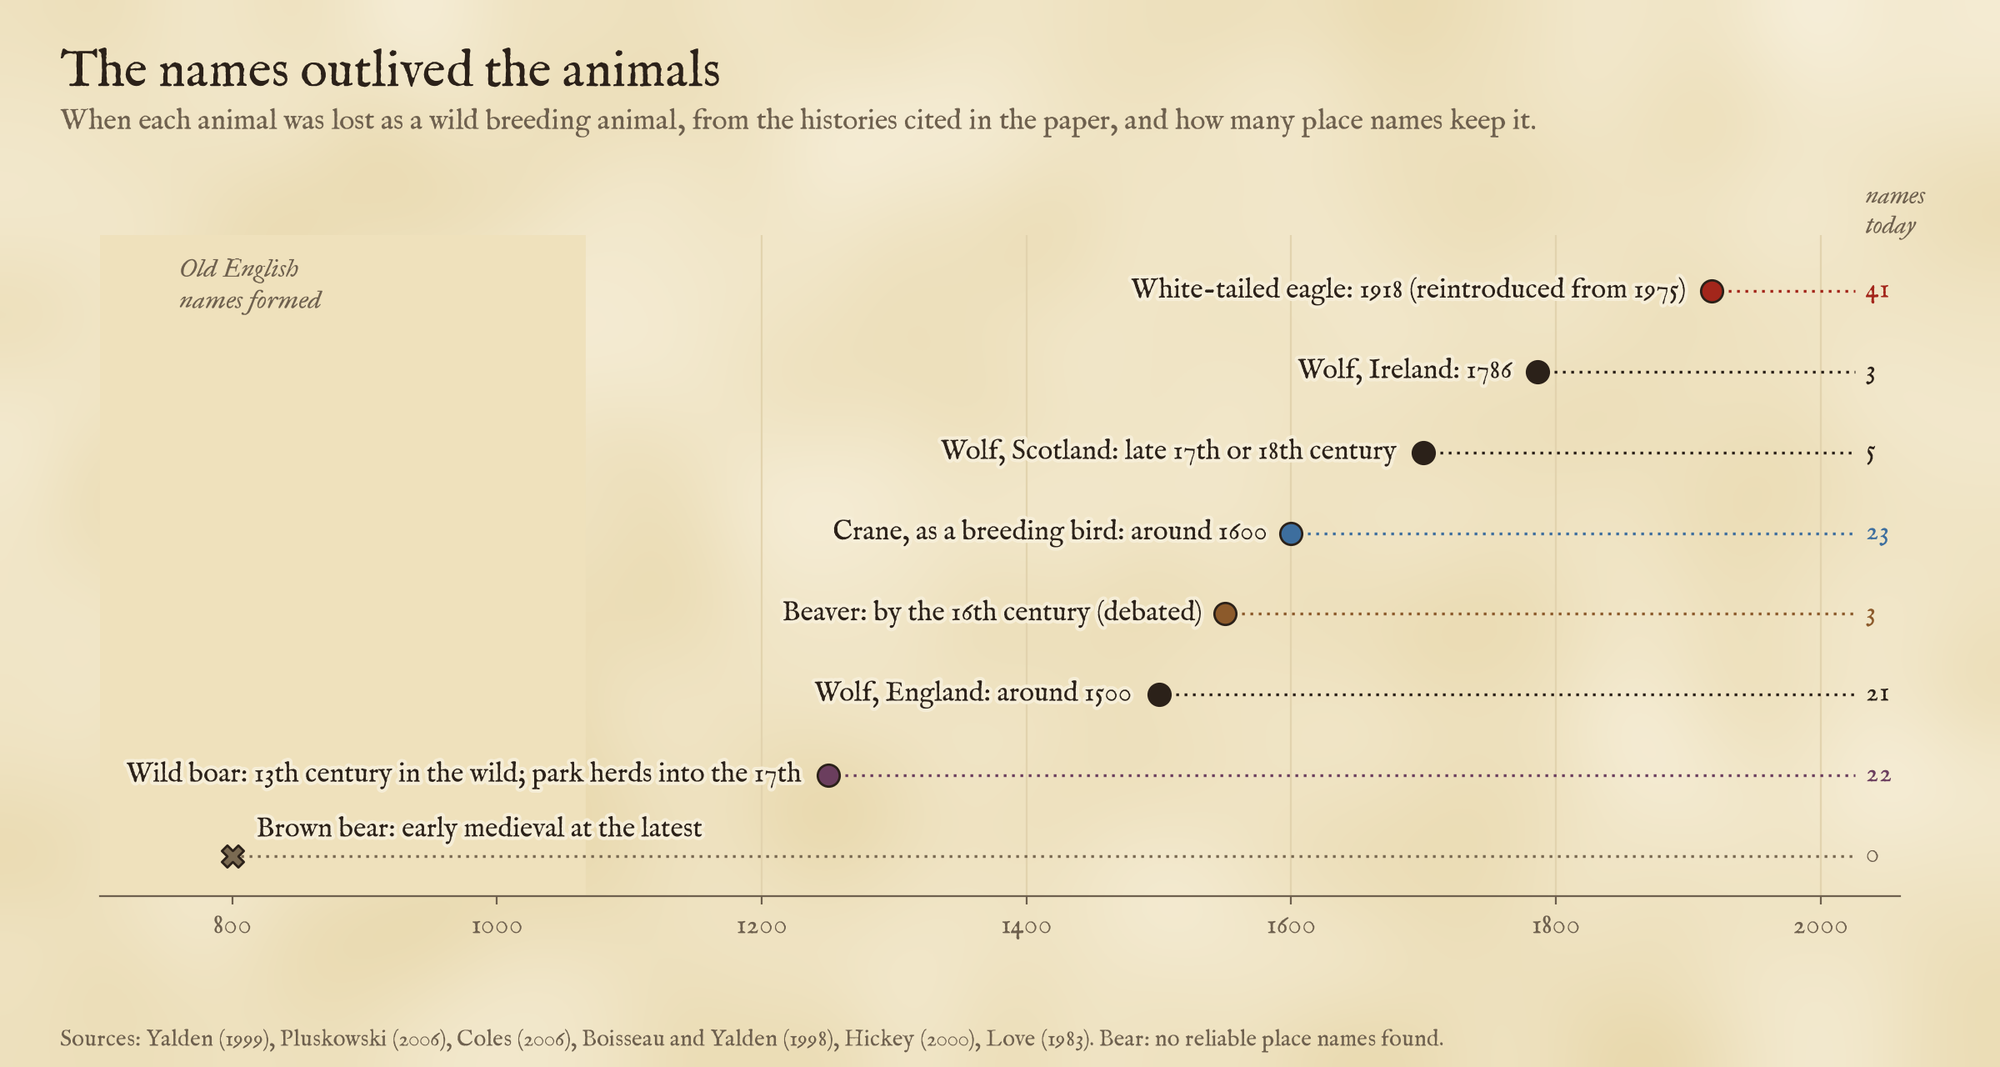
\includegraphics[width=\textwidth]{f_lost.png}
\caption{When each animal was lost in the wild, and the number of places keeping its name.}\label{fig:lost}\end{figure}

\begin{table}[tbp]\centering\small\caption{Some false friends removed by rule or in review.}\label{tab:ff}\begin{tabular}{llp{8.4cm}}\toprule Name & Looks like & Is\\\midrule
Wolverhampton & wolf & Wulfrun's high farm, after a woman's name\\
Eagle (Lincolnshire) & eagle & Old English ac-leah, oak wood\\
Eaglesham & eagle & Gaelic eaglais, a church\\
Swanage & swan & Old English swan, herdsmen\\
Roedean & roe deer & Old English ruh denu, rough valley\\
Brockley & badger & a brook, or a personal name\\
Cranagh & crane & Irish crann, a tree\\
Donnybrook & badger & Domhnach Broc, St Broc's church\\
\bottomrule\end{tabular}\end{table}

\begin{small}\begin{longtable}{R{2.2cm}R{1.3cm}R{2.6cm}R{3.7cm}R{2.7cm}l}\caption{The named rules: English and Norse settlement names read with an animal after the standard dictionaries (Mills 2011; Watts 2004; Ekwall 1960), the counties where they apply and the certainty given.}\label{tab:named}\\\toprule Name & Animal & Element & Meaning & Counties & Reading\\\midrule\endhead
Woolpit & Wolf & OE wulf-pytt & pit for trapping wolves & Suffolk & certain\\
Woolley & Wolf & OE wulf + lēah & wood or clearing frequented by wolves & West Yorkshire & certain\\
Woolley & Wolf & OE wulf + lēah & wood or clearing frequented by wolves (as the Yorkshire Woolley; not checked for this one) & any & probable\\
Ulpha & Wolf & ON ulfr + haugr & hill frequented by wolves & Cumbria & certain\\
Wolf's Castle & Wolf & Welsh Casblaidd, blaidd & the wolf's castle (Welsh Casblaidd) & Dyfed & probable\\
Beverley & Beaver & OE beofor + a stream name & beaver stream or beaver lodge & East Riding of Yorkshire & certain\\
Bevercotes & Beaver & OE beofor + cot & beavers' lodges, shelters for beavers & Nottinghamshire & certain\\
Beversbrook & Beaver & OE beofor + brōc & beavers' brook & Wiltshire & probable\\
Cranfield & Crane & OE cran + feld & open land frequented by cranes or herons & Bedfordshire & certain\\
Cranbrook & Crane & OE cran + brōc & brook frequented by cranes or herons & Kent & certain\\
Cranborne & Crane & OE cran + burna & stream frequented by cranes or herons & Dorset & certain\\
Cranbourne & Crane & OE cran + burna & stream frequented by cranes or herons & Berkshire & probable\\
Cranford & Crane & OE cran + ford & ford frequented by cranes or herons & Greater London, Northamptonshire & certain\\
Cranmore & Crane & OE cran + mere & pool frequented by cranes or herons & Somerset & certain\\
Cranwell & Crane & OE cran + wella & spring or stream frequented by cranes or herons & Lincolnshire & certain\\
Cranleigh & Crane & OE cran + lēah & clearing frequented by cranes or herons & Surrey & certain\\
Cransley & Crane & OE cran + lēah & clearing frequented by cranes or herons & Northamptonshire & probable\\
Tranmere & Crane & ON trani + melr & sandbank frequented by cranes & Merseyside & certain\\
Cranshaws & Crane & OE cran + sceaga & wood frequented by cranes or herons & Scottish Borders & probable\\
Arncliffe & Eagle & OE earn + clif & cliff frequented by eagles & North Yorkshire & certain\\
Earnley & Eagle & OE earn + lēah & wood or clearing frequented by eagles & West Sussex & certain\\
Arnold & Eagle & OE earn + halh & nook of land frequented by eagles & Nottinghamshire & certain\\
Arnold & Eagle & OE earn + halh & nook of land frequented by eagles & East Riding of Yorkshire & probable\\
Yarnscombe & Eagle & OE earn + cumb & valley of the eagles & Devon & probable\\
Ernesettle & Eagle & OE earn + setl & eagle's seat or eyrie & Devon & probable\\
Everley & Wild boar & OE eofor + lēah & wood or clearing frequented by wild boar & Wiltshire, North Yorkshire & certain\\
Eversley & Wild boar & OE eofor + lēah & wood or clearing of the wild boar & Hampshire & certain\\
Evershot & Wild boar & OE eofor + scēat & corner of land frequented by wild boar & Dorset & probable\\
Eversholt & Wild boar & OE eofor + holt & wood frequented by wild boar & Bedfordshire & probable\\
Everdon & Wild boar & OE eofor + dūn & hill frequented by wild boar & Northamptonshire & probable\\
Wildboarclough & Wild boar & ME wilde bor + OE clōh & ravine frequented by wild boar & Cheshire & certain\\
Hertford & Deer & OE heorot + ford & ford frequented by harts & Hertfordshire & certain\\
Hartlepool & Deer & OE heorot + ēg + pōl & pool by the hart island (Heruteu) & Durham & certain\\
Hartfield & Deer & OE heorot + feld & open land frequented by harts & East Sussex & certain\\
Hartley & Deer & OE heorot + lēah & wood or clearing frequented by harts & any & probable\\
Hartley Wintney & Deer & OE heorot + lēah & wood or clearing frequented by harts & Hampshire & certain\\
Hartford & Deer & OE heorot + ford & ford frequented by harts & Cheshire, Cambridgeshire, Northumberland & probable\\
Harthill & Deer & OE heorot + hyll & hill frequented by harts & South Yorkshire, Cheshire, North Lanarkshire & probable\\
Hartshead & Deer & OE heorot + hēafod & the hart's headland or hill & West Yorkshire & probable\\
Hartsop & Deer & OE heorot + hop & valley of the hart & Cumbria & certain\\
Hartshorne & Deer & OE heorot + horn & hart's horn, a hill shaped like one & Derbyshire & probable\\
Hartwell & Deer & OE heorot + wella & spring frequented by harts & Buckinghamshire, Northamptonshire & probable\\
Hartburn & Deer & OE heorot + burna & stream frequented by harts & Northumberland, Durham & probable\\
Hindhead & Deer & OE hind + hēafod & hill frequented by hinds & Surrey & certain\\
Hindley & Deer & OE hind + lēah & wood or clearing frequented by hinds & Greater Manchester & certain\\
Darley & Deer & OE dēor + lēah & wood or clearing frequented by deer & Derbyshire, North Yorkshire & probable\\
Durley & Deer & OE dēor + lēah & wood or clearing frequented by deer & Hampshire & certain\\
Deerhurst & Deer & OE dēor + hyrst & wooded hill frequented by deer & Gloucestershire & certain\\
Dyrham & Deer & OE dēor + hamm & enclosed valley or deer enclosure & Gloucestershire & certain\\
Dearham & Deer & OE dēor + hām or hamm & homestead or enclosure where deer are kept & Cumbria & probable\\
Brockhall & Badger & OE brocc + hol & badger holes (setts) & Northamptonshire & certain\\
Brockholes & Badger & OE brocc + hol & badger holes (setts) & West Yorkshire, Lancashire & certain\\
Foxley & Fox & OE fox + lēah & wood or clearing frequented by foxes & England & certain\\
Foxholes & Fox & OE fox + hol & fox holes, earths & North Yorkshire & certain\\
Foxearth & Fox & OE fox + eorth & fox's earth & Essex & certain\\
Foxcote & Fox & OE fox + cot & fox's earth or den & any & probable\\
Foxhall & Fox & OE fox + hol & fox hole & Suffolk & probable\\
Foxton & Fox & OE fox + denu or tūn & valley or farm frequented by foxes & Leicestershire, Cambridgeshire, Durham, North Yorkshire & probable\\
Catford & Wildcat & OE catt + ford & ford frequented by (wild) cats & Greater London & certain\\
Catcleugh & Wildcat & OE catt + clōh & ravine of the (wild) cats & Northumberland, Scottish Borders & probable\\
Catshill & Wildcat & OE catt + hyll & hill frequented by (wild) cats & Worcestershire & probable\\
Otterburn & Otter & OE otor + burna & otter stream & Northumberland, North Yorkshire & certain\\
Otterbourne & Otter & OE otor + burna & otter stream & Hampshire & certain\\
Ottery St Mary & Otter & OE otor + ēa (River Otter) & on the River Otter, 'otter stream' & Devon & certain\\
Otterton & Otter & OE otor + ēa + tūn (River Otter) & farm on the River Otter, 'otter stream' & Devon & certain\\
Leixlip & Salmon & ON lax + hlaup & salmon leap & any & certain\\
Swanmore & Swan & OE swan + mere & pool frequented by swans & Hampshire & probable\\
Swanbourne & Swan & OE swan + burna & stream frequented by swans & Buckinghamshire & probable\\
Gledhow & Kite & OE gleoda + hōh & hill spur frequented by kites & West Yorkshire & probable\\
\bottomrule\end{longtable}\end{small}

\section{Limitations}
A name records what someone noticed, feared or joked about when it was given, not a population; one wolf pit or crane-haunted pool tells us little about numbers. OpenStreetMap is a gazetteer of present-day points, uneven in coverage between regions and mappers, and almost without the field names and minor names where most wildlife names are recorded, which is why the counts here are far smaller than those from the county surveys \citep{aybes1995}. The dictionary readings are the standard ones but some are debated, and the individual etymologies were applied from the dictionaries without re-examining early spellings. The descriptive English and Scots names may honour a surname, an inn sign or a story rather than a living animal, and are marked probable. Gaelic and Welsh coverage depends on whether the Gaelic or Welsh form is the OpenStreetMap name or tagged; Wales in particular is under-counted. Ground heights are from 90 m terrain at the mapped point.

\section{Conclusion}
Read carefully, an open gazetteer gives a fair sketch of the animals in British and Irish place names: wolves on northern crags and in a few old English villages, cranes and beavers in English settlement names, eagles, ravens and boar in Gaelic hills, and the common animals in the later names of the land. The names have outlived the wolves, beavers, cranes and boar by four to eight centuries. Every rule, decision and name is published so that others can correct and extend the list.

\section*{Data and code availability}
The interactive map is at \url{https://maps.tristanhotham.com/animal-place-names/}. Code, the element list, the overrides and every candidate with its decision are at \url{https://github.com/Tristan-Hotham/animal-place-names} and archived with this paper at https://doi.org/10.5281/zenodo.24075293. The name tables are derived from OpenStreetMap (\copyright{} OpenStreetMap contributors) and released under the Open Database Licence; text and figures CC BY 4.0; code MIT. Ground heights from the AWS Terrain Tiles; county boundaries from the ONS (Open Government Licence v3.0).

\section*{AI statement}
I wrote the text, with drafting and editing assistance from Claude (Anthropic), which also helped prepare the analysis code. I reviewed and checked all text and results.

\begin{thebibliography}{20}
\bibitem[Aybes and Yalden(1995)]{aybes1995} Aybes, C. and Yalden, D. W. (1995) Place-name evidence for the former distribution and status of wolves and beavers in Britain. \textit{Mammal Review} 25, 201 to 227.
\bibitem[Bast and Buchhold(2017)]{bast2017} Bast, H. and Buchhold, B. (2017) QLever: a query engine for efficient SPARQL+Text search. \textit{Proceedings of the 26th ACM International Conference on Information and Knowledge Management (CIKM 2017)}, 647 to 656.
\bibitem[Boisseau and Yalden(1998)]{boisseau1998} Boisseau, S. and Yalden, D. W. (1998) The former status of the Crane \textit{Grus grus} in Britain. \textit{Ibis} 140(3), 482 to 500.
\bibitem[Coles(2006)]{coles2006} Coles, B. (2006) \textit{Beavers in Britain's Past}. WARP Occasional Paper 19. Oxford: Oxbow Books.
\bibitem[Ekwall(1960)]{ekwall1960} Ekwall, E. (1960) \textit{The Concise Oxford Dictionary of English Place-Names}, 4th edn. Oxford: Clarendon Press.
\bibitem[Gelling and Cole(2000)]{gelling2000} Gelling, M. and Cole, A. (2000) \textit{The Landscape of Place-Names}. Stamford: Shaun Tyas.
\bibitem[Hickey(2000)]{hickey2000} Hickey, K. (2000) A geographical perspective on the decline and extermination of the Irish wolf \textit{Canis lupus}: an initial assessment. \textit{Irish Geography} 33, 185 to 198.
\bibitem[Love(1983)]{love1983} Love, J. A. (1983) \textit{The Return of the Sea Eagle}. Cambridge: Cambridge University Press.
\bibitem[Mills(2011)]{mills2011} Mills, A. D. (2011) \textit{A Dictionary of British Place-Names}, revised edn. Oxford: Oxford University Press.
\bibitem[Owen and Morgan(2007)]{owen2007} Owen, H. W. and Morgan, R. (2007) \textit{Dictionary of the Place-Names of Wales}. Llandysul: Gomer.
\bibitem[Pluskowski(2006)]{pluskowski2006} Pluskowski, A. (2006) \textit{Wolves and the Wilderness in the Middle Ages}. Woodbridge: Boydell Press.
\bibitem[Watson(1926)]{watson1926} Watson, W. J. (1926) \textit{The History of the Celtic Place-Names of Scotland}. Edinburgh: Blackwood.
\bibitem[Watts(2004)]{watts2004} Watts, V. (ed.) (2004) \textit{The Cambridge Dictionary of English Place-Names}. Cambridge: Cambridge University Press.
\bibitem[Yalden(1999)]{yalden1999} Yalden, D. (1999) \textit{The History of British Mammals}. London: T. and A. D. Poyser.
\end{thebibliography}
\end{document}
